\documentclass[aps,prd,nofootinbib,twocolumn,reprint,superscriptaddress,showpacs,showkeys,longbibliography]{revtex4-1}
\pdfoutput=1
\usepackage {amsmath}
\usepackage {amssymb}
\usepackage {amsfonts}
\usepackage {amsthm}
\usepackage {mathrsfs}
\usepackage {natbib}
\usepackage {latexsym}
\usepackage {graphicx}
\usepackage {dsfont}
\usepackage {txfonts}
\usepackage {rotating}
\usepackage {wasysym}
\usepackage {multirow}
\usepackage {hhline}
\usepackage {graphicx}
\usepackage {hyperref}
\usepackage[dvipsnames,usenames]{color}
\usepackage {bm}
\usepackage{appendix}
\usepackage{acronym}
\usepackage{dcolumn}   % needed for some tables
\usepackage{enumitem}
\usepackage{bigdelim}
\usepackage {url}
\usepackage{caption}
\usepackage {subcaption}
\usepackage{multirow}
% REMINDER TO CHRIS: subcaption.sty might need to be included,
% or else the package removed; isn't universally installed -- GDM

\usepackage{framed}

%% ----- macros lifted from aastex.cls
\newcommand\arcdeg{\mbox{$^\circ$}}%
\newcommand\arcmin{\mbox{$^\prime$}}%
\newcommand{\bra}[1]{\langle #1|}
\newcommand{\ket}[1]{|#1\rangle}
\newcommand{\braket}[2]{\langle #1|#2\rangle}

%% ----- some handy shortcuts
\newcommand{\dcc}{LIGO-XXXXXXXXX}
%% -----
\newcommand{\cm}[1]{\textbf{\textcolor{red}{CM: #1}}}
\newcommand{\dg}[1]{\textbf{\textcolor{blue}{DG: #1}}}
%% ----- Version that makes the comments disappear
%% -----
\newcommand\marginnote[1]{%
    \mbox{}\marginpar{\raggedleft\hspace{0pt}\footnotesize\textcolor{green}
\raggedright\hspace{0pt}\footnotesize\textcolor{green}
    {#1}}}
%% ----- macros for cross-references

%% ----- input git-version tag
\input{tag.tex}

%% ----- define shorthand variables

\begin{document}

\title{Quantum matched filtering}

% NOTE TO EVERYBODY: we should decide on whether to make
% names full or initialized -- GDM
\author{Sijia Gao}
\email{s.gao.2@research.gla.ac.uk}
\affiliation{SUPA, School of Physics and Astronomy, University of Glasgow, Glasgow G12 8QQ, United Kingdom}
\author{Fergus Hayes}
\email{f.hayes.1@research.gla.ac.uk}
\affiliation{SUPA, School of Physics and Astronomy, University of Glasgow, Glasgow G12 8QQ, United Kingdom}
\author{Sarah Croke}
\affiliation{SUPA, School of Physics and Astronomy, University of Glasgow, Glasgow G12 8QQ, United Kingdom}
\author{J.~Veitch}
\affiliation{SUPA, School of Physics and Astronomy, University of Glasgow, Glasgow G12 8QQ, United Kingdom}
\author{C.~Messenger}
\affiliation{SUPA, School of Physics and Astronomy, University of Glasgow, Glasgow G12 8QQ, United Kingdom}

\date{\today}
\date{\commitDATE\\\mbox{\small{\commitID} \commitSTATUS}\\\mbox{\dcc}}

\begin{abstract}
We did a quantum thing
\end{abstract} 

\maketitle

\acrodef{NS}[NS]{Neutron Star}
\acrodef{GW}[GW]{gravitational-wave}

%%%%%%%%%%%%%%%%%%%%%%%%%%%%%%%%%%%%%%%%%%%%%%%%
%%%%%%%%%%%%%%%%%%%%%%%%%%%%%%%%%%%%%%%%%%%%%%%%
\section{Introduction}\label{sec:intro}

\begin{itemize}
\item GW introduction
\item Quantum computing introduction
\item summary of what this paper intends to do 
\end{itemize}

%%%%%%%%%%%%%%%%%%%%%%%%%%%%%%%%%%%%%%%%%%%%%%%%
%%%%%%%%%%%%%%%%%%%%%%%%%%%%%%%%%%%%%%%%%%%%%%%%
\section{Background}\label{sec:background}

\subsection{Matched-filtering}

\begin{itemize}
\item derive matched-filtering as a semi-optimal statistic
\item What problem it solves
\end{itemize}

\subsection{Grovers algorithm}

The search for the closest matching template or templates in gravitational wave detection may be thought of as belonging to the class of generic search problems. For such problems, we wish to identify a ``marked" solution, i.e. one satisfying a certain set of criteria, from within an unstructured database of possible solutions. In fact, any problem for which it is easy to verify a solution, but difficult to find one may be thought of as a search problem, also known as NP problems. Indeed for certain NP-hard problems the best known classical algorithms offer limited improvement over brute-force search.\cite{bennett1997strengths} In the case of match filtering, we can consider the database to be made up of all possible templates, and we are searching for one or more for which the match with the data is above a specified threshold. Typically the number of templates is much larger than the complexity of checking whether a given template is a match, and is the limiting factor determining the time needed for match filtering in gravitational wave data analysis. For a database with $N$ entries and exactly one good solution, we need to check $\frac{N}{2}$ entries on average before finding the marked entry. In other words, for generic search problems, the required search time for a classical algorithm is $O(N)$ \cite{barnett2009quantum}. Grover's algorithm, proposed by Lov Grover in 1996, provides a polynomial speed-up for these problems, finding a solution in $O(\sqrt{N})$ search time \cite{grover1996fast}. It was later proved that this is asymptotically optimal; $\Omega(\sqrt{N})$ queries are required for a quantum algorithm to succeed with high probability \cite{bennett1997strengths}.
\newline\newline Grover's algorithm establishes a gap in query complexity between classical and quantum computers, in an oracle model. That is, it assumes that we have access to an oracle, a``black box" which computes a desired function, but not necessarily a description of the function itself. The query complexity is then given by the number of calls required to the oracle. To cast the search problem as an oracle problem, we can define a function $f(x)$, according to which $f(x)=1$ if and only if $x$ is our marked entry in the database, %\smc{\sout{also known as the basis state,} (this is only true in the quantum case - we're not talking about the quantum case yet - I've moved this to introduce the basis state a bit later)}
otherwise $f(x)=0$. In the quantum case, we imagine we have a quantum black box or oracle $U_f$ that can perform the following procedure:
\begin{equation}
    \label{Ufa}
    U_f: \ket{x}\otimes\ket{b}\longmapsto\ket{x}\ket{b \oplus f(x)},
\end{equation}
where $\ket{x}$ is the input register containing the input $x$ encoded as a computational basis state, and $\ket{b}$ is an ancilla register into which the output is written. We see that for $b=0$ the evaluation of the function is contained here. The key difference in the quantum case is that we can query the oracle in superposition, that is, we can prepare the input register in a superposition over all input states. In the rest of this section we outline Grover's algorithm, before addressing the problem of how to construct an oracle for match filtering in the following section. Grover's algorithm is covered in several introductory quantum computing texts, e.g. \cite{barnett2009quantum, nielsen2002quantum,kaye2007introduction}. We begin by noting that if we prepare our ancilla register in the state $\ket{-}=\frac{1}{\sqrt{2}}(\ket{0}-\ket{1})$, the operation given in Eq.~\ref{Ufa} is equivalent to the following procedure on the input register alone:
\begin{equation}
    \label{Uf}
    U_f: \ket{x}\longmapsto(-1)^{f(x)}\ket{x}.
\end{equation}
Although in the actual algorithm we need the ancilla register for the oracle, in the following discussion, we prefer to use Eq.~\ref{Uf} for the oracle evaluation for simplicity. 
\newline\newline Considering the problem of the search of the closest template, we represent the position of each template in the database as a computational basis state $\ket{i}$ and prepare the input register in an equal superposition over all positions $\ket{s}$. Suppose there are $N$ templates, the input register can be expressed as:
\begin{equation}
    \label{soo}
    \ket{s}=\frac{1}{\sqrt{N}}\sum^{N-1}_{0} \ket{i},
\end{equation}
where $\frac{1}{\sqrt{N}}$ represents the amplitude of each state in the superposition. This ensures that each state has the same probability of $\frac{1}{N}$ of being found. We shall start with the simplest situation where there is exactly one desired match, $\ket{w}$. The rest of the basis, i.e. the bad solutions can be marked as $\ket{s'}$, which are perpendicular to the state $\ket{w}$. We can rewrite the input state $\ket{s}$ using the new expression as:
\begin{equation}
    \label{so}
    \ket{s}=\frac{1}{\sqrt{N}}\ket{w}+\frac{\sqrt{N}-1}{\sqrt{N}}\ket{s'}.
\end{equation}
It is obvious that in order to decrease the number of enquiries needed to achieve the correct solution, we need to increase the amplitude of the state $\ket{w}$. We can also use a two dimensional vector graph to represent the input register $\ket{s}$ as shown in Fig.~\ref{2d0}A, where the angle is defined as:
\begin{equation}
\label{theta}
   \theta=\arcsin\braket{w|s}=\arcsin {\frac{1}{\sqrt{N}}}.
\end{equation}
Our goal, in the context, is to rotate state $\ket{s}$ to make it parallel, or closer to parallel, to state $\ket{w}$. After applying the oracle $U_f$, the input state $\ket{s}$ becomes:
\begin{equation}
    \label{ufs}
    U_f\ket{s}=-\frac{1}{\sqrt{N}}\ket{w}+\frac{\sqrt{N}-1}{\sqrt{N}}\ket{s'},
\end{equation}
which is equivalent to flip the input state $\ket{s}$ with respect to the horizontal axis $\ket{s'}$, as represented in Fig.~\ref{2d0}B. This procedure itself however, does not make the desired state $\ket{w}$ more favourable in the measurement. Therefore, an additional diffusion unitary operator is applied as the third step, which is defined as:
\begin{equation}
    \label{Us}
    U_s=2\ket{s}\bra{s}-\hat{\rm I},
\end{equation}
where $\hat{\rm I}$ is the identity operator. The action of this operator would result in the state:
\begin{equation}
    \label{usufs}
    U_sU_f\ket{s}=(1-\frac{4}{\sqrt{N}})\ket{s'}+\frac{1}{\sqrt{N}}(3-\frac{4}{N})\ket{w}.
\end{equation}
From Eq.~\ref{usufs} which it is obvious that the probability of $\ket{w}$ being the outcome of a measurement has increased from $\frac{1}{N}$ to $\frac{1}{N}(3-\frac{4}{N})^2$. This shows the speedup of Grover's algorithm as long as we have more than one template. If we decompose Eq.~\ref{ufs} into $\ket{s}$ and its orthogonal state, $\ket{s_\perp}$, as $U_f\ket{s}=a\ket{s}+b\ket{s_\perp}$, Eq.~\ref{usufs} can also be rewritten as:
\begin{equation}
    \label{usufsp}
    U_sU_f\ket{s}=a\ket{s}-b\ket{s_\perp}.
\end{equation}
This shows the diffusion operator is equivalent of flipping the $U_f\ket{s}$ state with respect to the $\ket{s}$ state, as shown in Fig.~\ref{2d0}C.
\begin{figure}[h]
{\caption{A) The red line represents the input initial state $\ket{s}$ represented as a vector in a plane spanned by the desired match $\ket{s}$ and undesired match $\ket{s'}$. B) The blue line represents the result of the oracle acting on the initial state $\ket{s}$ which now represented by the red dot dashed line. C) The green line represents the result of the diffusion operator acting on the result state in B, $U_f\ket{s}$ which now represented by the blue dotted line.   }\label{2d0}}
{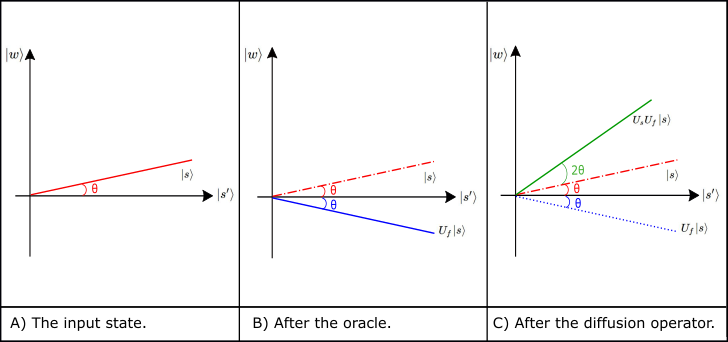
\includegraphics[width=0.45\textwidth]{Grover.png}}
 \end{figure}
If we define the grover operator $\hat{G}$ as:
\begin{equation}
    \label{Gdef}
    \hat{G}= U_sU_f,
\end{equation}
it is obvious from the previous discussion that it is equivalent to a rotation operator in the two-dimensional space spanned by $\ket{w}$ and $\ket{s'}$:
\begin{equation}
    \label{Gmatrix}
    \hat{G}=\begin{pmatrix}
\cos{2\theta} & \sin{2\theta} \\
-\sin{2\theta} & \cos{2\theta} 
\end{pmatrix}.
\end{equation}
After applying the Grover's operator $k$ times, the input state would become:
\begin{equation}
    \label{Gks}
    \hat{G}^k \ket{s}= \sin{\big((2k+1)\theta\big)}\ket{w}+\cos{\big((2k+1)\theta\big)}\ket{s'}.
\end{equation}
In order to maximise the probability of finding the desired match $\ket{w}$, we need to maximise its amplitude $\sin{\big((2k+1)\theta\big)}$. In other words, we need to apply the Grover's algorithm $k$ times that $(2k+1)\theta=\frac{\pi}{2}$. This means that:
\begin{equation}
\label{k}
    k\approx\frac{\pi}{4}\sqrt{N},
\end{equation}
for large number of templates.
\newline \newline
If there exists multiple matches, we can rewrite the input state $\ket{s_t}$ as:
\begin{equation}
    \label{som}
    \ket{s_t}=\sqrt{\frac{t}{N}}\ket{w_t}+\frac{\sqrt{N}-\sqrt{t}}{\sqrt{N}}\ket{s'_t},
\end{equation}
where $t$ is the number of desired templates, $\ket{w_t}$ refers to all the desired templates and $\ket{s'_t}$ are all the undesired templates. In this case, in the two-dimensional space spanned by $\ket{w_t}$ and $\ket{s'_t}$, state $\ket{s_t}$ is represented by a vector with an angle $\theta_t$ defined as:
\begin{equation}
\label{thetat}
   \theta_t=\arcsin\braket{w_t|s_t}=\arcsin {\sqrt{\frac{t}{N}}}. 
\end{equation}
Still, in order to maximise the amplitude of the desired templates, we need to apply the Grover's algorithm $k_t$ times that $(2k_t+1)\theta_t=\frac{\pi}{2}$. If the number $t$ of the desired templates are known, it is obvious that
\begin{equation}
\label{kt}
    k_t\approx\frac{\pi}{4}\sqrt{\frac{N}{t}}.
\end{equation}
However, in most cases we do not know the number of the desired templates. In this case we can use a variant of Grover's algorithm known as quantum counting\cite{brassard1998quantum}. As we have discussed above, each step in Grover's algorithm is a rotation through an angle $2 \theta_k$, which is now unknown. Quantum phase estimation is a well-known quantum algorithm which allows us to estimate just such an unknown angle of rotation. We don't describe this in detail here, but refer the interested reader to \cite{nielsen2002quantum}. For large number of templates N, the phase estimation part does not add extra complexity in the computation time \cite{brassard1998quantum}. In fact, it can find the period of a function in a time $O(log^3P)$, where P is a n-bit number representing the period. The extra computation time is polynomial in n.\cite{barnett2009quantum}

%%%%%%%%%%%%%%%%%%%%%%%%%%%%%%%%%%%%%%%%%%%%%%%%
%%%%%%%%%%%%%%%%%%%%%%%%%%%%%%%%%%%%%%%%%%%%%%%%
\section{Quantum psuedo-code}\label{sec:psuedocode}

\begin{itemize}
\item How to construct the Oracle
\item A counting argument for the complexity - templates are indices
\item discuss template erasure
\item actually show the psuedo-code representation
\end{itemize}

%%%%%%%%%%%%%%%%%%%%%%%%%%%%%%%%%%%%%%%%%%%%%%%%
%%%%%%%%%%%%%%%%%%%%%%%%%%%%%%%%%%%%%%%%%%%%%%%%
\section{Example using Qiskit}\label{sec:qizkitexample}

\begin{itemize}
\item define model (small number of qubits and exact matching)
\item focus on results
\end{itemize}

%%%%%%%%%%%%%%%%%%%%%%%%%%%%%%%%%%%%%%%%%%%%%%%%
%%%%%%%%%%%%%%%%%%%%%%%%%%%%%%%%%%%%%%%%%%%%%%%%
\section{Example on Sine wave (python)}\label{sec:sineexample}

\begin{itemize}
\item continuous wave GW signal motivation
\item why we don't just use the QFT? Our real CW signals (and CBCs) are not monochromatic
\item Define sine wave model
\item focus on showing results - number of steps taken
\end{itemize}

%%%%%%%%%%%%%%%%%%%%%%%%%%%%%%%%%%%%%%%%%%%%%%%%
%%%%%%%%%%%%%%%%%%%%%%%%%%%%%%%%%%%%%%%%%%%%%%%%
\section{CBC application example}\label{sec:cbcexample}

\begin{itemize}
\item define the CBC waveform model
\item focus on results - compare to GWOSC GW150914 data
\item make the number of steps clear (~ root N operations)
\end{itemize}

%%%%%%%%%%%%%%%%%%%%%%%%%%%%%%%%%%%%%%%%%%%%%%%%
%%%%%%%%%%%%%%%%%%%%%%%%%%%%%%%%%%%%%%%%%%%%%%%%
\section{Practical considerations}\label{sec:intro}

Discuss things about practicalities for the future. How many qubits are needed
etc.. 

\begin{itemize}
\item space requirements on quantum computer
\item describe the current state of the art in quantum processors
\end{itemize}

%%%%%%%%%%%%%%%%%%%%%%%%%%%%%%%%%%%%%%%%%%%%%%%%
%%%%%%%%%%%%%%%%%%%%%%%%%%%%%%%%%%%%%%%%%%%%%%%%
\section{Discussion}\label{sec:discussion}

\begin{itemize}
\item Summarise the entire paper first
\item highlight the parts of interest to Quantum and GW fields separately
\item Discuss limitations of what we've done
\item Talk about future work
\item Talk about the future of Quantum computers and the future GW data
analysis challenges
\item It's not just GWs though - data analysis searches in general
\end{itemize}

%%%%%%%%%%%%%%%%%%%%%%%%%%%%%%%%%%%%%%%%%%%%%%%%
\begin{acknowledgments}
We would liek the thank \ldots
\end{acknowledgments}


%%%%%%%%%%%%%%%%%%%%%%%%%%%%%%%%%%%%%%%%%%%%%%%%
\appendix

%%%%%%%%%%%%%%%%%%%%%%%%%%%%%%%%%%%%%%%%%%%%%%%%
%%%%%%%%%%%%%%%%%%%%%%%%%%%%%%%%%%%%%%%%%%%%%%%%
\section{Optional Appendix\label{sec:appendix}}


% Create the reference section using BibTeX:
\bibliography{masterbib}

\end{document}